\documentclass[11pt,a4paper]{article}
\usepackage[margin=2.3cm]{geometry}
\usepackage[T1]{fontenc}
\usepackage{textcomp}
\input{glyphtounicode}
\pdfgentounicode=1
\usepackage{lmodern}
\usepackage{xcolor}
\usepackage{listings}
\usepackage{tcolorbox}
\usepackage{booktabs}
\usepackage{array}
\usepackage{tikz}
\usepackage{hyperref}
\hypersetup{colorlinks=true, linkcolor=blue!50!black, citecolor=green!40!black}

\definecolor{codebg}{RGB}{248,248,245}
\lstset{
  language=C, basicstyle=\ttfamily\footnotesize, backgroundcolor=\color{codebg},
  keywordstyle=\color{blue!60!black}\bfseries, commentstyle=\color{green!45!black}\itshape,
  stringstyle=\color{red!60!black}, numbers=none, upquote=true,
  frame=single, rulecolor=\color{gray!40}, breaklines=true, columns=fullflexible,
  keepspaces=true, showstringspaces=false
}
\lstdefinestyle{sh}{language=bash, backgroundcolor=\color{black!5}}

\newtcolorbox{keyidea}{colback=blue!4, colframe=blue!45!black, title=Key ideas, fonttitle=\bfseries\small}
\newtcolorbox{experiment}{colback=orange!5, colframe=orange!70!black, title=Experiment, fonttitle=\bfseries\small}

\title{\textbf{OpenMP --- Lesson 7}\\[4pt]\large Data in and out of a region: \texttt{firstprivate}, \texttt{lastprivate}, \texttt{default(none)}}
\author{Gustavo Lozano}
\date{November 2026}

\begin{document}
\maketitle

\noindent\textit{\small Source: Chapman, Jost \& van der Pas~\cite{chapman}, Ch.~4
``OpenMP Language Features'' (data-sharing attribute clauses).}

\section{The idea}
In Lesson~2 we saw that \texttt{private(x)} gives each thread its own copy of
\texttt{x}. But that copy is cut off from the original in both directions:
\begin{itemize}
  \item \textbf{in}: the copy starts \emph{uninitialised}, it does not receive the value
        \texttt{x} had before the region;
  \item \textbf{out}: the copy is \emph{discarded} at the end, nothing goes back to
        \texttt{x}.
\end{itemize}
Two clauses open one of these directions each, and a third one protects you from
forgetting to decide.

\begin{center}
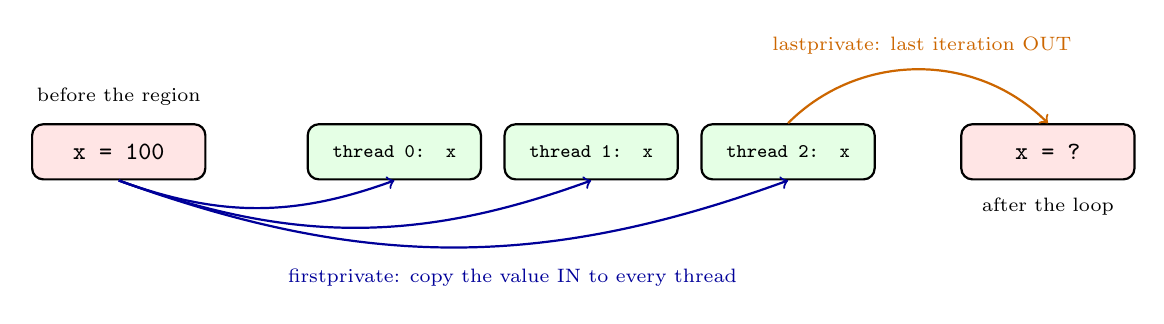
\begin{tikzpicture}[thick, box/.style={draw, rounded corners, minimum width=2.2cm, minimum height=0.7cm, font=\small\ttfamily}]
  \node[box, fill=red!10] (before) at (0,0) {x = 100};
  \node[font=\scriptsize] at (0,0.7) {before the region};
  \foreach \i/\x in {0/3.5,1/6,2/8.5} {
    \node[box, fill=green!10] (t\i) at (\x,0) {};
    \node[font=\scriptsize\ttfamily] at (\x,0) {thread \i: x};
    \draw[->, blue!60!black] (before.south) to[bend right=20] (t\i.south);
  }
  \node[font=\scriptsize, blue!60!black] at (5,-1.6) {firstprivate: copy the value IN to every thread};
  \node[box, fill=red!10] (after) at (11.8,0) {x = ?};
  \node[font=\scriptsize] at (11.8,-0.7) {after the loop};
  \draw[->, orange!80!black] (t2.north) to[bend left=45] (after.north);
  \node[font=\scriptsize, orange!80!black] at (10.2,1.35) {lastprivate: last iteration OUT};
\end{tikzpicture}
\end{center}

\section{The three clauses}
\begin{center}
\small
\begin{tabular}{@{}>{\raggedright\arraybackslash}p{3.4cm}>{\raggedright\arraybackslash}p{11.8cm}@{}}
\toprule
Clause & Meaning \\ \midrule
\texttt{private(x)} & private copy, \textbf{uninitialised}; discarded at the end (Lesson 2) \\
\texttt{firstprivate(x)} & private copy, \textbf{initialised} with the value of \texttt{x}
  before the region \\
\texttt{lastprivate(x)} & private copy; after a \texttt{for} (or \texttt{sections}),
  \texttt{x} receives the value from the \textbf{sequentially last} iteration
  (\texttt{i = n-1}), whichever thread ran it \\
\texttt{default(none)} & no implicit rules: every variable used in the region and declared
  outside it must appear in a clause, or the program \textbf{does not compile} \\
\bottomrule
\end{tabular}
\end{center}

\paragraph{Why \texttt{default(none)} matters.} Most OpenMP bugs are a variable that is
shared by default when it should be private (Lesson~2). With \texttt{default(none)} you
must write down a decision for every variable, and the compiler checks that you did.
Using it in every parallel region is a widely recommended habit.

\section{The code}
\lstinputlisting[title=\texttt{data\_clauses.c}]{data_clauses.c}

\begin{lstlisting}[style=sh]
gcc -Wall -fopenmp -o data_clauses data_clauses.c
OMP_NUM_THREADS=4 ./data_clauses
\end{lstlisting}
Typical output (line order in Part 1 will differ):
\begin{lstlisting}[style=sh]
--- Part 1: firstprivate ---
  thread 0: offset = 100
  thread 1: offset = 101
  thread 2: offset = 102
  thread 3: offset = 103
  after the region: offset = 100
--- Part 2: lastprivate ---
  after the loop: last = 49   (a[n-1] = 49)
\end{lstlisting}

\begin{keyidea}
\begin{itemize}
  \item Every thread starts from 100 because of \texttt{firstprivate}, and each changes
        only its own copy.
  \item After the region \texttt{offset} is still 100: private copies never flow back.
  \item \texttt{last = 49 = 7*7}: the value from \texttt{i = n-1}, the last iteration in
        \emph{sequential} order, not from the thread that finished last.
  \item \texttt{a} and \texttt{n} are listed as \texttt{shared}: \texttt{n} is only read,
        and each thread writes different elements of \texttt{a}, so there is no race.
\end{itemize}
\end{keyidea}

\section{The experiment}
\begin{experiment}
\textbf{Question:} what changes when each clause is removed or replaced?\\
Make one change at a time, recompile with \texttt{-Wall}, run, then undo it.
\begin{enumerate}
  \item In Part~1 replace \texttt{firstprivate(offset)} by \texttt{private(offset)}.
        Read the compiler warning, then run.
  \item In Part~2 replace \texttt{lastprivate(last)} by \texttt{private(last)}. Run.
  \item In Part~2 replace \texttt{shared(a, n)} by \texttt{shared(a)}. Compile.
\end{enumerate}
\textbf{What to observe and answer.}
\begin{enumerate}
  \item With \texttt{private}, what values do the threads print? Why does the compiler warn?
  \item Without \texttt{lastprivate}, what is \texttt{last} after the loop? Why?
  \item What does the compiler say in step 3? What would have happened without
        \texttt{default(none)}?
\end{enumerate}
\end{experiment}

\paragraph{Answers (read after trying).}
(1)~Garbage, for example \texttt{32740, 32741, \ldots}: each thread adds its id to an
uninitialised copy. GCC warns that \texttt{offset} is used uninitialised. The value
before the region never reaches the threads.
(2)~\texttt{last = -1}, its value before the loop. The private copies held 49 and other
values, but with \texttt{private} they are discarded and nothing is copied out.
(3)~\texttt{error: 'n' not specified in enclosing 'parallel'}. Without
\texttt{default(none)}, \texttt{n} would silently be shared, which here happens to be
correct. The point is that the compiler forces \emph{you} to decide; in Lesson~2 the
silent default was exactly what caused the race.

\paragraph{Next lesson.} False sharing: why threads that write to \emph{different}
variables can still slow each other down (Chapman et al., Ch.~5).

\begin{thebibliography}{9}
\bibitem{chapman} B.~Chapman, G.~Jost, and R.~van der Pas. \emph{Using OpenMP: Portable
  Shared Memory Parallel Programming}. MIT Press, Cambridge, MA, 2007.
\end{thebibliography}
\end{document}
